\hypertarget{project-velocity}{%
\subsubsection{Project Velocity}\label{project-velocity}}

Question: What is the development speed for an organization?

\hypertarget{description}{%
\paragraph{Description}\label{description}}

Project velocity is the number of issues, the number of pull requests,
volume of commits, and number of contributors as an indicator of
'innovation'.

\hypertarget{objectives}{%
\paragraph{Objectives}\label{objectives}}

Gives an Open Source Program Office (OSPO) manager a way to compare the
project velocity across a portfolio of projects.

The OSPO manager can use the Project Velocity metric to:

\begin{itemize}
\tightlist
\item
  Report project velocity of open source projects vs in-house projects
\item
  Compare project velocity across a portfolio of projects
\item
  Identify which projects grow beyond internal contributors (when
  filtering internal vs. external contributors)
\item
  Identify promising areas in which to get involved
\item
  Highlight areas likely to be the successful platforms over the next
  several years
\end{itemize}

\href{https://www.cncf.io/blog/2017/06/05/30-highest-velocity-open-source-projects}{See
Example}

\hypertarget{implementation}{%
\paragraph{Implementation}\label{implementation}}

Base metrics include:

\begin{itemize}
\tightlist
\item
  \href{https://github.com/chaoss/wg-evolution/blob/master/metrics/Issues_Closed.md}{issues
  closed}
\item
  \href{https://github.com/chaoss/wg-evolution/blob/master/metrics/Reviews.md}{number
  of reviews}
\item
  \href{https://github.com/chaoss/wg-evolution/blob/master/metrics/Code_Changes.md}{\#
  of code changes}
\item
  \href{https://github.com/chaoss/wg-risk/blob/master/metrics/Committers.md}{\#
  of committers}
\end{itemize}

\hypertarget{filters}{%
\subparagraph{Filters}\label{filters}}

\begin{itemize}
\tightlist
\item
  Internal vs external contributors
\item
  Project sources (e.g., internal repositories, open-source
  repositories, and competitor open-source repositories)
\item
  Time
\end{itemize}

\hypertarget{visualizations}{%
\subparagraph{Visualizations}\label{visualizations}}

\begin{itemize}
\tightlist
\item
  X-Axis: Logarithmic scale for Code Changes
\item
  Y-Axis: Logarithmic scale of Sum of Number of Issues and Number of
  Reviews
\item
  Dot-size: Committers
\item
  Dots are projects
\end{itemize}

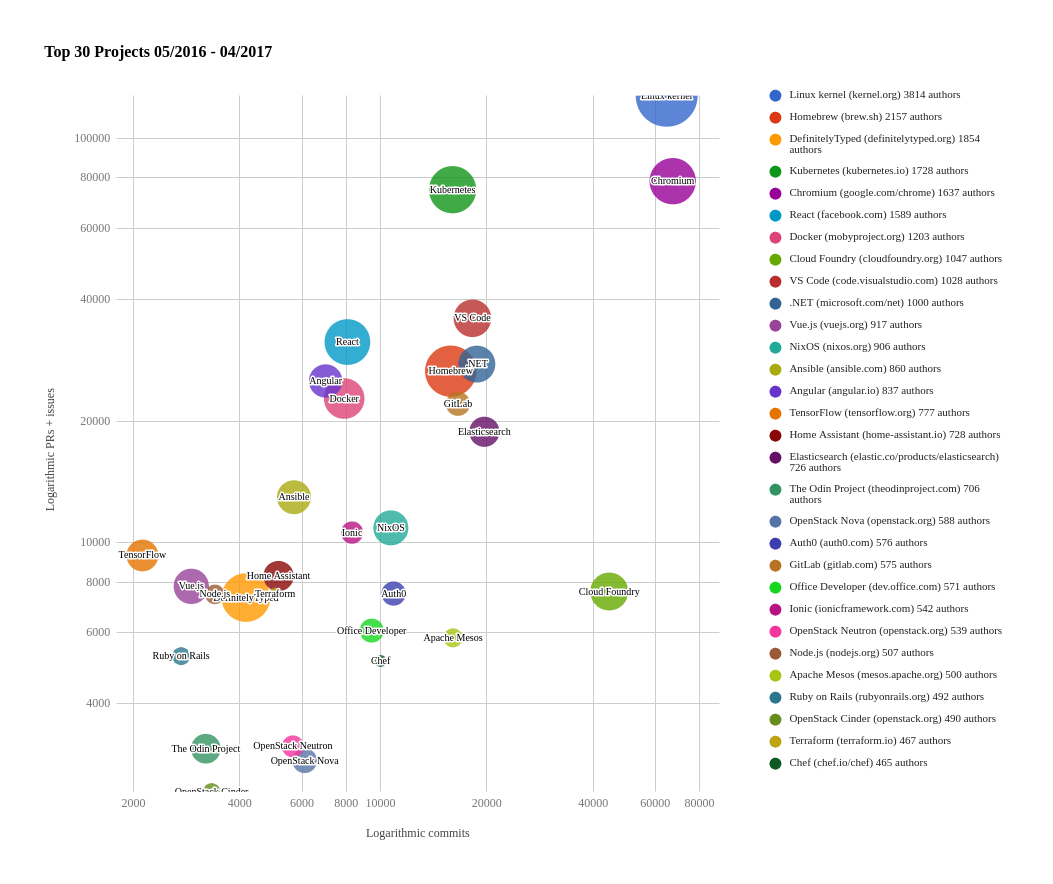
\includegraphics{images/project-velocity_visualization.png}

\href{https://www.cncf.io/blog/2017/06/05/30-highest-velocity-open-source-projects/}{From
CNCF}

\hypertarget{tools-providing-the-metric}{%
\subparagraph{Tools providing the
Metric}\label{tools-providing-the-metric}}

\begin{itemize}
\tightlist
\item
  CNCF - \url{https://github.com/cncf/velocity}
\end{itemize}

\hypertarget{references}{%
\paragraph{References}\label{references}}

\begin{itemize}
\tightlist
\item
  \href{https://www.threefivetwo.com/blog/can-open-source-innovation-work-in-the-enterprise}{Can
  Open Source Innovation work in the Enterprise?}
\item
  \href{https://www.nearform.com/blog/want-a-high-performing-culture-make-way-for-open-innovation}{Open
  Innovation for a High Performance Culture}
\item
  \href{https://www.cio.com/article/3213146/open-source-is-powering-the-digital-enterprise.html}{Open
  Source for the Digital Enterprise}
\item
  \href{https://www.cncf.io/blog/2017/06/05/30-highest-velocity-open-source-projects}{Highest
  Velocity Open Source Projects}
\end{itemize}
